\documentclass[sigconf,nonacm,prologue,table]{acmart}
\usepackage{listings}

%% labels
%% sections:    "sec"
%% definitions: "def"
%% equations:   "eq"
%% figures:     "fig"
%% tables:      "tab"

%% packages
\usepackage{amsmath}
\usepackage{pgfplots}
\usepackage{subcaption}
\usepackage{commath}
\usepackage[utf8]{inputenc}
\usetikzlibrary{positioning, arrows.meta, shapes, calc}
\usepackage{titlesec}
%% \usepackage{tikz}

\pagenumbering{arabic}

%% hide ACM reference
\settopmatter{printacmref=false}

%% hide copyright
\renewcommand\footnotetextcopyrightpermission[1]{}

%% \pagestyle{plain}
\settopmatter{printfolios=true}

\numberwithin{equation}{section}

\theoremstyle{definition}
\newtheorem{definition}{Definition}

\theoremstyle{remark}
\newtheorem*{remark}{Remark}

\captionsetup[subfigure]{
    labelfont=bf,
    textfont=normalfont,
}
\renewcommand{\thesubfigure}{\Roman{subfigure}}

\definecolor{rowA}{gray}{0.9}
\definecolor{rowB}{gray}{0.8}

\newcommand{\rplus}{\mathbb{R}_{\geq 0}}
\newcommand{\rpos}{\mathbb{R}_{>0}}

\begin{document}
\title{Doppler: A liquidity bootstrapping ecosystem [Draft]}
\subtitle{Aug 2024}
\date{Aug 2024}

\author{Austin Adams}
\affiliation{}
\email{austin@whetstone.cc}

\begin{teaserfigure}
\caption*{
    \hspace{\textwidth}
    }
\end{teaserfigure}

\renewcommand{\shortauthors}{Adams}

\begin{abstract}
Doppler is a liquidity bootstrapping ecosystem that facilitates liquidity provision by introducing a new primitive: a dutch-auction dynamic bonding curve, which is used to source initial two-sided liquidity. This mechanism is a self-executing and non-custodial Uniswap v4 hook designed for automated initial price discovery for arbitrary assets. Additionally, Doppler provides infrastructure to allow ecosystems to go from token deployment to an arbitrary liquid generalized automated market maker without user intervention.
\end{abstract}

\maketitle

\section{Introduction} \label{sec:introduction}
The rise of automated market makers (AMMs), such as the Uniswap Protocol \cite{Adams21}, and the subsequent shift in market structure towards automated pricing algorithms has resulted in an exponential increase in the number of traded onchain assets, with more than 910,000\footnote{Source: https://dune.com/queries/3891972} unique traded assets created as of writing. Despite this, token projects continue to struggle to bootstrap liquidity, and oftentimes must outsource to automated liquidity management protocols or onchain market making desks, which generally take a sizeable portion of the provided assets. 

However, one benefit of blockchain-based ecosystems is that they allow for programmable markets. Just as the Uniswap Protocol is designed to facilitate trading through an $xy=k$ model, a similar model could be created to bootstrap liquidity. Indeed, we have already seen such projects on both Solana, Tron, and Ethereum.

Traditionally, the problem with creating new market structures is the difficulty of creating customized AMM protocols, which require expertise and significant time and capital investment. However, the forthcoming \textsc{Uniswap v4} \cite{Adams23} improves the customization and integrator experience of AMMs by introducing hooks, which can execute developer-defined logic at specific points in the transaction's lifecycle. While \textsc{Uniswap v3} \cite{Adams21} focused on optimizing the most common trading flow, \textsc{Uniswap v4} allows custom market structure models for specialized tasks.

\section{Background} 
\label{sec:Background}

The rise of AMMs and resulting increase of trade-able assets present their own challenges. Creating liquid pools is a common source of friction for users and token projects. For example, \textsc{Uniswap v2} \cite{Adams20} requires token projects to provide two assets to create a fully liquid pool. Token projects must therefore not only acquire the tokens needed to fund both sides of the pool, which can be a substantial financial barrier, but also take a stance on the price of both assets and run the risk of incurring significant losses if that stance is wrong. While projects such as \textsc{Uniswap v3} \cite{Adams21} have utilized single-sided liquidity, which requires only one asset, token projects must still take an initial stance on the asset’s price. 

Creating liquid pools is further complicated by the need to find the initial market price, which is both difficult and a very impactful problem for liquidity provision. If the initial price is too low, then significant capital is lost from the instantaneous arbitrage. If the price is too high, then no trading will occur. 

A fundamental nature of permissionless systems, like email or TCP, is the vast amount of value-less user generated content. This type of market structure is formalized in Oh \cite{oh2023digital}, which models non-fungible tokens (NFTs) as "digital Veblen goods." The implication of this model is that the purchasing of an asset greatly increases likelihood that a product is valuable.

This market dynamic is well-supported by static bonding curves implemented in projects like friendtech. Bonding curves start assets with cheap prices with the next trade being marginally more expensive than the previous. However, these protocols can run into significant issues from programmatic bots, who buy these cheap assets and instantly sell if the price increases. This strategy is very low risk, because the bonding curves are static. The initial buyers of the tokens cannot lose any money. The price either goes up as new users buy, allowing the initial buyers to sell and collect a profit, or (if no one bought) they sell at the original price they paid (due to the static bonding curve). Single-sided liquidity bootstrapping from Intuitive Launch Pool functions similarly to this model, utilizing concentrated liquidity math as the bonding curve.

Another problem plaguing onchain markets is inconsistent or malicious token code. Because the ERC20 is a standard, there are many implementations that fit the standard, making them available for trading. Many liquidity bootstrapping projects solve this problem by providing a singular token contract with known code and invariants.

Doppler provides a dutch-auction dynamic bonding curves liquidity bootstrapping hook and a token factory to create ERC20s with known bytecode. This allows ecosystems to go from token deployment to liquid generalized automated market maker, like Uniswap v2 or Uniswap v4, without user intervention. 

\begin{itemize}
    \item \emph{Dutch-auction Dynamic Bonding Curves}: Price discovery of assets is facilitated through the dutch-auction dynamic bonding curve. This mechanism is built on top of \textsc{Uniswap v4}, facilitating automated price discovery and auctioning without intervention. Additionally, user experience should be identical to and supported by the current swapping experience. 
    \item \emph{Token contract Factory}: The ecosystem utilizes a token contract factory to deploy ERC20s with known bytecode. This bytecode removes many of the malicious implementations prevalent in the EVM ecosystems and allows 3rd party interfaces to quickly check bytecode. Additionally, this factory and hook combine to enforce invariants on token trading.
    \item \emph{Direct to \textsc{generalized liquidity}}: Once the required tokens are bootstrapped to create a liquid pool, the \textsc{Uniswap v4} hook contract deposits the funds directly into a generalized AMM without intervention. However, unlike other liquidity bootstrapping implementations, the underlying LP share tokens are not burned. In future versions, users can choose between \textsc{Uniswap v2}, a \textsc{CFMM on Uniswap v4}, or any arbitrary \textsc{Uniswap Protocol} pools.
    \item \emph{Time-locked liquidity}: Liquidity tokens for the generalized liquidity pool are time-locked initially, but can be withdrawn at a later date. This is to ensure that a community around that token can optionally utilize these funds at a later date.
\end{itemize}

The following sections provide in-depth explanations of each part of the token deployment ecosystem.

\section{Dutch-auction Dynamic Bonding Curves} 
\label{sec:bonding}

\emph{Dutch-auction Dynamic Bonding Curves} blend together two well-studied mechanisms in blockchain-based markets - dutch auctions and bonding curves. 

\subsection{Background}

Dutch auctions are a well-understood auction format, and have been studied deeply for onchain markets in pieces such as Frankie (2022) \cite{frankie2022gda} and Moallemi (2024) \cite{moallemi2024loss}. Dutch auctions are descending price auctions, where the auction starts at a high price and decays until a market clearing price is found. They are generally utilized within onchain markets due to their efficient implementation and "shill-proof" properties \cite{komo2024shillproofauctions}. To expand on this, in blockchain-based markets, bidding both reveals private information their about bids to all other market participants and the cost of bidding is non-zero (due to gas). This means when bidding a bidder essentially pays to give all other parties free private information about their bid. This causes drag on market efficiency. Dutch auctions also allow a fixed payoff from bidding, which creates a straightforward assessment for market participants on if they want to bid (revealing information to the rest of the market). 

On the other hand, bonding curves are another widely used blockchain-based markets primitive, which attempts to mimic the laws of supply and demand. As previously stated, static bonding curves have significant issues around determining the optimal starting levels. Too low a starting price, and significant value is lost due to the instantaneous arbitrage. Additionally, this value is lost to programmatic users who will instantly dump on other users, causing losses for users who desire long-term exposure to that ecosystem. For context, instantaneous arbitrage has cost token deployers over +\$100 million dollars on Ethereum mainnet over the last year\footnote{Source: https://dune.com/queries/3682272/6193594}. Likewise, instantaneous arbitrage and MEV have cost more than \$400m from users on pumpdotfun on Solana\footnote{Source: https://x.com/0xngmi/status/1823399442306801974}. 
Too high and trades never occur, but this is heavily mitigated by the dutch auction mechanism.

\subsection{Implementation}

The dutch-auction dynamic bonding curve has two phases
\begin{itemize}
    \item Rapid price decrease until an initial market clearing price is found
    \item Once a lower bound price is found, the expected price ramps up slowly using the dynamic bonding curve
\end{itemize}

 The optimal price curve is shown below. The price of the marginal token rapidly decreases until users begin buying, and the bonding curve behavior begins. This market behavior encourages the starting price of the dutch auction to be higher than "the market price", limiting losses from instantaneous arbitrage.
 
 It is important to note that if the price were to start "too low", the descending price auction would not occur, and regular dynamic bonding curve behavior would begin. There is no requirement in this mechanism for the descending price behavior - it is simply encouraged to maximize eventual liquidity. However, a significant price movement would cause the bonding curves to shift upward in a process that will be described in a later section.

\begin{figure}[htb]
    \label{fig:price_curve}
    \centering
    \begin{tikzpicture}
    \draw[help lines, color=gray!30, dashed] (0,0) grid (6.9,6.9);
    \draw[->,ultra thick] (0,0)--(7,0) node[right]{$time$};
    \draw[->,ultra thick] (0,0)--(0,7) node[above]{$price$};
    \draw[->, line width=0.5mm] (1,5) .. controls (2,2) .. (7,6); 
    \end{tikzpicture}
    \caption{\textbf{Optimal price curve}}
\end{figure}

\subsubsection{Liquidity Provision}

In order to minimize losses to instantaneous arbitrage, \verb|Doppler| streams liquidity into the pool at a configurable rate at each time. We define this liquidity at time $t$ as $\lambda_t$. In the current implementation, we stream a constant amount of liquidity into the pool at the start of each epoch. However, this could be adapted to arbitrary liquidity functions.

In order to facilitate optimal price movement, Doppler also keeps track of $\hat{\lambda_t}$, which tracks the realized amount of "net-sold" tokens within the system. "Net-sold" tokens is defined as the number of tokens that are held outside of the bonding curve. We utilize the difference between realized liquidity vs. expected liquidity to adjust the bonding curve's price over time. 

\subsubsection{Dutch Auction}

The dutch auction handles the decrease in price of tokens within the system. To start, the beginning price and end price of the dutch auction behavior is configurable by the interface that submits the trade. A interface may adjust these parameters depending on the expected starting price, potential volatility of the token, or based on broader market conditions. 

Similar to other dutch auction protocols like UniswapX \cite{adamsuniswapx} or 1inch Fusion \cite{1inchfusion}, Doppler uses a step-wise decaying function. In practice, due to \verb|tickSpacing| in \textsc{Uniswap v4}, the price may not actually decay until it has passed a \verb|tickSpacing|. 

\begin{figure}[htb]
    \label{fig:tick_decay}
    \centering
    \begin{tikzpicture}
    \draw[help lines, color=gray!30, dashed] (0,0) grid (5.9,5.9);
    \draw[->,ultra thick] (0,0)--(6,0) node[right]{$time$};
    \draw[->,ultra thick] (0,0)--(0,6) node[above]{$tick$};
    \draw[thick] (0,5) -- (1,5) node[above, right] {$\verb|maxTick|$};;
    \draw[thick]  (1,5) -- (1,4);
    \draw[thick]  (1,4) -- (2,4);
    \draw[thick]  (2,4) -- (2,3);
    \draw[thick]  (2,3) -- (3,3);
    \draw[thick]  (3,3) -- (3,2);
    \draw[thick]  (3,2) -- (4,2);
    \draw[thick]  (4,2) -- (4,1);
    \draw[thick]  (4,1) -- (5,1) node[above, right] {$\verb|minTick|$};
    \end{tikzpicture}
    \caption{\textbf{Target tick decay over time}} 
\end{figure}

Notice that the y-axis in Figure 2 says \verb|tick|. Due to implementation details of \textsc{Uniswap v4}, it is easier to decay the price in log-space. This is implemented through a linear decay of the underlying ticks from a given \verb|maxTick| to a given \verb|minTick|, which are then mapped into the price using concentrated liquidity math. 

Ideally, the decay should never reach \verb|minTick|, as the bonding curve (described below) should take over price discovery. If the end of the sale time is reached and the required proceeds are not met, users are refunded a pro-rata share of the pool holdings if under a minimum threshold. Above this threshold will cause the liquidity to be sent to \textsc{Uniswap v2} in the current design. The natural state of the pool is decaying to \verb|minTick|, which will occur if no tokens are purchased.

To support price movements caused by both the dutch auction and the dynamic bonding curve, the hook contract keeps an \verb|tickAccumulator| that tracks the tick changes applied by the two mechanisms.

Since we are linearly dutch auctioning, we can define the max decrease as such

\begin{equation}
    maxDelta = \frac{maxTick - minTick}{endingTime - startingTime} \cdot epochLength
\end{equation}

At each curve re-balance, the hook calculates expected amount of tokens from the liquidity function, $\lambda_t$, sold from the previous epoch to the current and the realized amount sold, $\hat{\lambda_t}$. There are three states depending on the amount of tokens that are sold

\begin{equation}
    tickDelta_t := \begin{cases} 
          maxDelta & \hat{\lambda_t} - \lambda_t \leq 0 \\
          \frac{maxDelta \cdot \hat{\lambda_t}}{\lambda_t} & 0 < \hat{\lambda_t} < \lambda_t \\
          tickDelta_{u,t} & \hat{\lambda_t} \geq \lambda_t
       \end{cases} 
\end{equation}
Note that $tickDelta_{u,t}$ will be defined in the Bonding Curve section. 

The \verb|tickDelta| is added to the \verb|tickAccumulator| during the rebalance of the curve, which is the accumulation of each \verb|tickDelta| from start to time $t$.

\begin{equation}
    tickAccumulator_t = \sum^t_{i=0} tickDelta_i 
\end{equation}

If the \verb|tickDelta| is 0, then either the expected number of tokens were sold.

\subsubsection{Dynamic Bonding Curves} 

The dutch auction attempts to decay until the market finds the "market clearing" bonding curve. The decay from the dutch auction acts like an impulse downward, which is countered by buy pressure (which raises the price), while the upward target price of the pool is determined by current active bonding curve. We refer to the current active bonding curve as the bonding curve that the pool is checking its current price against. 

\begin{figure}[H]
    \centering
    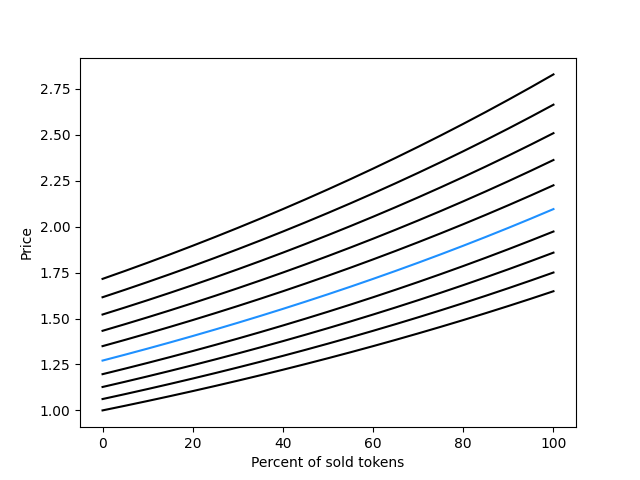
\includegraphics[scale=0.45]{images/curves.png} \caption{\textbf{Dynamic Bonding Curves with $\gamma$ = 500}}
\end{figure}

First, we define the origin tick of the bonding curve, $\tau_t$. To calculate this, Doppler takes the \verb|startingTick| and adds the \verb|tickAccumulator|. Note that the \verb|startingTick| is either \verb|minTick| or \verb|maxTick| depending on if the sold token is \verb|token0| or \verb|token1|.

\begin{equation}
    \tau_{t} = startingTick + tickAccumulator_t
\end{equation}

Above you can see an example of a collection of bonding curves, with the current active one in blue. The current bonding curve $b_c(t)$ can be calculated at any time from the origin tick ($\tau_t$), a growth parameter ($\gamma$), and the elapsed time ($t$). 

\begin{equation}
    b_c(t) = \gamma \cdot (t / t_{max}) + \tau_{t}
\end{equation}

Notice that $\tau_t$ is also the bottom/start of the bonding curve and the slope of the bonding curve is given by $\gamma$. A higher $\gamma$ means that the bonding curve is steeper. Using the \textsc{Uniswap v4} concentrated liquidity math, the tick can be converted to price.

\begin{equation}
    p(t) = 1.0001^{b_c(t)}
\end{equation}

Checking the surrounding bonding curves is also trivial as they are a constant \verb|tickSpacing| away. The current bonding curve is the position utilized by the pool for liquidity provision.

As time progresses in the pool, the current price must drift upward or downward, thus the desired bonding curve may change. To calculate when we should change the bonding curve, we can calculate the indifference curve between the current bonding curve against its two surrounding curves. Let $\tau_{t}$ be the current starting \verb|tick| at time $t$. We can define the two boundary curves, $b_u(t)$ and $b_l(t)$

\begin{equation} \label{eq:upperboundry}
    b_u(t) = \gamma \cdot (t / t_{max}) + (\tau_{t} + tickSpacing / 2)
\end{equation}
\begin{equation} \label{eq:lowerboundry}
    b_l(t) = \gamma \cdot (t / t_{max}) + (\tau_{t} - tickSpacing / 2)
\end{equation}

At the end of the epoch, if there was enough or extra tokens sold, we then want to increase the current target bonding curve. In this case, We calculate the current spot position of pool, $i_c$, against the expected position on the bonding curve.

\begin{equation} 
   tickDelta_{u,t} = i_c - (\gamma \cdot (t / t_{max}) + \tau_t)
\end{equation} 

We then adjust the \verb|tickDelta| to be on a boundary defined by the \verb|tickSpacing| of the pool. This adjustment functions similarly to the indifference curves defined above.

\subsubsection{Position Strategy}

As previously described, \verb|Doppler| streams liquidity into the pool according to a pre-described formula $\lambda_t$. At each time period, \verb|Doppler| calculates the current amount of net-sold tokens, $\hat{\lambda_t}$ and the amount of tokens expected to be sold before the next epoch, $\lambda_{t+1}$. This amount of tokens is placed between the current tick, $i_c$ and the $b_c(t+1)$, which is the expected price of the pool at the next epoch. If $(\lambda_{t+1} - \hat{\lambda_t}) \leq 0$, this position is skipped.

Next, \verb|Doppler| calculates the expected amount of tokens sold between the next epoch $\lambda_{t+1}$ and the epoch after that $\lambda_{t+2}$. This liquidity is placed from either the top of the previous position or the current tick, and then to the $\gamma + \tau_t$, which is the top of the current bonding curve.

\subsubsection{Implementation Details} 

In \textsc{Uniswap v4}, $i_c$ is the current tick of the pool, determined through swapping. It is reasonable to ask if the pool bonding curve can be manipulated as $i_c$ is the spot price of the pool. 

Because the bonding curve is set in the \verb|beforeSwap| hook in \textsc{Uniswap v4}, the hook is able to respond to manipulations during their execution (and cannot be censored). Because of this, a manipulator would lose funds from the shifting of the bonding curve, functioning as limit orders which are a strong mitigation to manipulations. Additionally, the portion of the bonding curve that allows selling of the tokens back may disjoint itself in a process described below.

On Ethereum mainnet (or any chain without strong censorship resistance\cite{fox2023}), it is possible for multiple slots in a row to be purchased by a manipulator (multi-block MEV). This actor could censor buy transactions until the price of the pool decreases, locking in an  lower than market clearing price. A mitigation to this attack is that the price increase defined by the provided $\gamma$ should always be greater than \verb|maxDelta|. Additionally, a chain could be utilized with censorship resistance, meaning that that this censorship would always lose to in priority gas auction for a backrun. This is because the rebalances occur before the first trade of the epoch, meaning that manipulations would need to span blocks and epochs. In practice, extractive multi-block MEV is rare on Ethereum mainnet due to validators' incentives. This problem is not present on any chain with censorship resistance, like most Layer 2 protocols.

One key design decision is to keep both tokens in the pool fully liquid at all times. However, it is possible that the current bonding curve does not have enough quote token liquidity to support $b_c(t)$ from $\tau_t$ to $i_c$. This is likely from a misspecified starting price or rapid price appreciation (either manipulations or naturally). 

If the pool is in this state, then we utilize two different $b_c(t)$ above and below the current $i_c$. The only way to move the $i_c$ down would be selling tokens into the pool. In this state, we create a one \verb|tickSpacing|-wide position at the price which supports a theoretical liquidation of the entire net-sold liquidity amount, $\hat{\lambda_t}$. This is to discourage run behavior and give a common clearing price to all users who wish to sell back their tokens.

\section{Token-contract Factory}

While utilizing a set standard for token contracts is not a new innovation, the design of the token contract factory is made to optimize for interface developer experience. However, the token factory is not required to utilize the \verb|Uniswap v4| hook, so this will only serve as an overview.

\subsection{Background}
While the ERC20 token contracts have a set of standards for most common actions, the specification is designed to be as minimalist as possible. For example, many tokens trading on decentralized markets today utilize a "fee-on-transfer" (FoT) mechanism, which adds an additional fee for every trade. There is no common standard for this flow.

Lack of a FoT standard causes interfaces issues when setting slippage limits (the minimum amount of tokens received for the swap). In practice, this requires interfaces to check if transferring a token adds an additional fee, which is not always accurate and requires chain RPC calls.

Another prevalent issue on EVM-based blockchains is that the token contracts are entirely programmable, which can lead to bad outcomes for end users. For example, some malicious ERC20 contracts allow wallets to mint infinite amounts of the new token, which is then used to rug-pull the token. Many popular apps for trading newly created tokens will use heuristics to check the token contract for common scams, but this leads to an unwinnable arms race for these interfaces. 

It would be better to instead assert that the token contract came from a known source with known bytecode. This flow is known as a "factory-pair" model and is commonly supported in decentralized finance applications.

\subsection{Implementation}

Doppler provides a factory that deploys ERC20s with bytecode that includes invariants. On initialization, users can provide a number of feature flags to set the adjust how the token works. These features all have standard "getters" for interfaces to check these token flags.

While not an exhaustive list, some of the feature flags are:

\begin{itemize}
    \item Fee on token transfers
    \item Buy taxes (and exclusions)
    \item Sell taxes (and exclusions)
    \item Various types of distributions of those taxes
    \item Initial airdrops to wallets
\end{itemize}

Additionally, the portion of the tokens that are typically reserved for the developers of the token project are not given until the token project is fully liquid. Significant losses to retail users have come from sells in the bonding curve phase. A developer aiming for longer term support should be able to wait for the token project leaving the bonding curve. Plus, once a token project leaves the bonding curve, the price impact of a developer selling their shares is not as impactful due to the liquidity not being concentrated. We have also seen many token projects recover from the original developer selling their shares when the token project is liquid. 

\section{Protocol and Interface Fees}

For providing this ecosystem, Doppler takes a small protocol fee, which is by default on.  Optionally, interfaces can additionally take an additional additive fee. The total fees taken is capped at 100 bps. Doppler takes 10 bps or 17.6\% of the interface fee, whichever is higher. This effectively means that interfaces can take up to a 85 bps fee. The Protocol and Interface fee are generated based on the LP fee from the hook itself. 

By enshrining a large interface fee, this will incentivize interfaces to coalesce around a single standard. This coalescence will improve trading safety and discoverability for other projects using the standard. It will also allow interfaces to focus on what they are best at producing instead of focusing on the market structure.

\section{Summary}

Doppler is a liquidity bootstrapping ecosystem, designed on top of \textsc{Uniswap v4} for efficient price discovery of assets. Doppler additionally provides safe standards for token trading, including a factory for the deployment of ERC20s with known bytecode.

\bibliographystyle{ACM-Reference-Format}
\bibliography{main}

\section{Disclaimers}

\textbf{No Legal, Financial, or Investment Advice.} This document does not constitute legal advice, financial advice, investment advice, trading advice, or a recommendation of any kind by Doppler, its affiliates, or any of their respective officers, directors, managers, employees, agents, advisors, or consultants. No information contained herein should be relied upon as the basis for any investment decision, contract, or any other decision regarding engagement with Doppler or any of its projects.

\textbf{Forward-Looking Statements.} This document may contain forward-looking statements based on assumptions and beliefs of Doppler, its officers, or its affiliates. These statements are subject to known and unknown risks, uncertainties, and other factors, many of which are outside Doppler's control, that may cause actual outcomes to differ materially from the projections or expectations set forth in such statements. Doppler makes no obligation to update or revise any forward-looking statements to reflect subsequent events, developments, or changes in circumstances after the date on which such statements were made, except as required by law.
\end{document}
\endinput